\section{Design}
\label{sec:design}

\begin{figure}[t]
\centering
\IfFileExists{figures/fig_design.pdf}{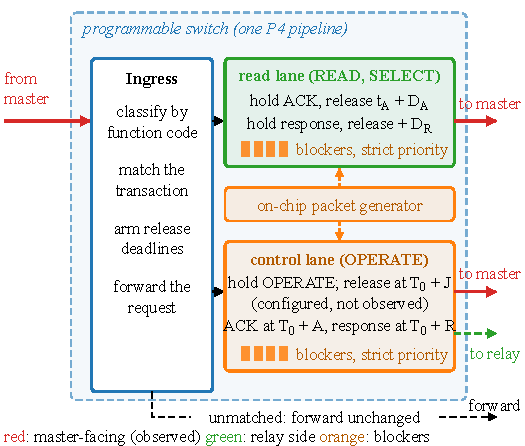
\includegraphics{figures/fig_design}}{\figplaceholder{Design overview. Ingress records the request arrival $T_0$ and arms the deadlines $T_0{+}A$ and $T_0{+}R$. Two independent scheduling lanes: the read lane holds the acknowledgment and the response; the control lane holds the operate response. Each held packet waits behind a reservoir of blocker packets that a strict-priority scheduler drains first; the on-chip packet generator fills the reservoirs. Unmatched traffic bypasses the treatment.}}
\caption{Design of \sysname. Ingress anchors every deadline to the request arrival $T_0$; two
independent scheduling lanes hold the read and the control answers; reservoirs of blocker packets,
drained by a strict-priority scheduler, realize the deadlines without a timer.}
\label{fig:design}
\end{figure}

In Figure~\ref{fig:design}, we present the design of \sysname. A request enters the switch from the
master. The program records the request's arrival time and forwards the request to the relay. When the
relay answers, the program holds the answer in a switch queue and releases it at a fixed offset from
the recorded request time, so the master sees a timing that the policy sets rather than one the
outstation produces. Because the read and the control answers must not interfere, each is held on its
own scheduling lane. The rest of this section presents the four mechanisms this requires.

\textbf{Anchoring deadlines to the request.} A held packet must leave at a fixed offset from the
request, but the switch has no general-purpose timer. On the request, the program records an ingress
timestamp $T_0$ and arms two deadlines from the policy offsets $A$ and $R$,
\begin{equation}
\label{eq:release}
t_{\mathrm{ack}} = T_0 + A, \qquad t_{\mathrm{resp}} = T_0 + R ,
\end{equation}
at which it releases the acknowledgment and the response to the master. Consequently, the interval the
adversary measures is
\begin{equation}
\label{eq:clrt}
\Delta = t_{\mathrm{resp}} - t_{\mathrm{ack}} = R - A ,
\end{equation}
a policy value, in place of the native interval $c$ that the outstation's internal processing produces.

Let $a$ and $r$ denote the arrival times, relative to $T_0$, of the relay's acknowledgment and
response. Because the switch can delay a packet but cannot emit one before it exists, the offsets are
admissible only if
\begin{equation}
\label{eq:admissible}
A \ge a_{\max}, \qquad R \ge r_{\max} ,
\end{equation}
where $a_{\max}$ and $r_{\max}$ bound the native arrivals over the traffic to be protected. Since
$\Delta$ is then constant for every transaction, the observable no longer varies with $c$.

\textbf{Security Argument.} The anchor matters as much as the offsets. Because the relay's own
acknowledgment arrives at $T_0+a$, a deadline of the form $T_0+a+D$ would make the observable depend on
$a$ and carry the device's own timing into it. Anchoring to $T_0$, which the adversary already
observes, removes that dependence and makes~(\ref{eq:clrt}) independent of the outstation. We check
this against a mutant design that arms the deadline at the relay's acknowledgment
(Section~\ref{sec:eval}).

\textbf{Reservoirs as data-plane timers.} To realize a deadline from packet scheduling alone, a held
packet waits in its queue behind a reservoir of small blocker packets. Since a strict-priority
scheduler drains the blockers first, the held packet cannot leave until its reservoir empties. If
$\tau$ is the time to drain one blocker, a reservoir of $K$ blockers holds a packet for $K\tau$, so the
control plane realizes a deadline $D$ with
\begin{equation}
\label{eq:reservoir}
K = \left\lceil D / \tau \right\rceil ,
\end{equation}
and sizes the reservoirs of~(\ref{eq:release}) with $D = A$ and $D = R$. The switch's on-chip packet generator fills
the reservoirs, and it never generates traffic toward the master or the relay. A tag byte distinguishes
the generator profiles, such that a read and a control trigger different reservoirs without ambiguity.

\textbf{Two independent scheduling lanes.} The read answer and the control answer are held at the same
time, and a single lane would serialize them: whichever holds longer would delay the other and reshape
the timing the policy fixed. Consequently, \sysname gives each treatment its own internal
recirculation lane and its own queues, so the two holds proceed independently.

\textbf{Normalizing the control command.} A control uses Select-before-Operate, so the adversary times
the interval between the OPERATE and its response. \sysname admits the OPERATE once, holds it, and
releases it to the relay at an internal delay $J$, while the acknowledgment and the echo the master
sees are placed at fixed offsets from the OPERATE's arrival $T_0$, as in~(\ref{eq:release}). The
observable operation time is therefore
\begin{equation}
\label{eq:optime}
O = (T_0 + R) - (T_0 + A) = R - A ,
\end{equation}
in which $J$ does not appear.

\textbf{Security Argument.} By~(\ref{eq:optime}), the observable operation time does not vary with $J$,
because the master-visible events are anchored to the OPERATE's arrival rather than to the relay's
answer. Consequently, an adversary that measures the operation time learns the policy, not the physical
device behind the command. Because $J$ is absent from~(\ref{eq:optime}), the adversary also cannot
subtract a known offset to recover the device's own timing.

\textbf{Failing open.} A defense on the control path must not become an availability risk. If a
transaction does not match an armed treatment, \sysname forwards it unchanged rather than dropping it.
Consequently, an unexpected exchange loses its protection but not its delivery, and the switch
actuates no output of its own.

\textbf{Byte preservation.} \sysname only holds and forwards packets. Because it neither pads a
response, injects a packet into the protected exchange, nor edits a DNP3 field, every byte the master
reassembles is the byte the relay produced, and the payload's cyclic redundancy checks remain valid.
